\documentclass{standalone}
\usepackage{tikz}
\usetikzlibrary{patterns, positioning}


\begin{document}
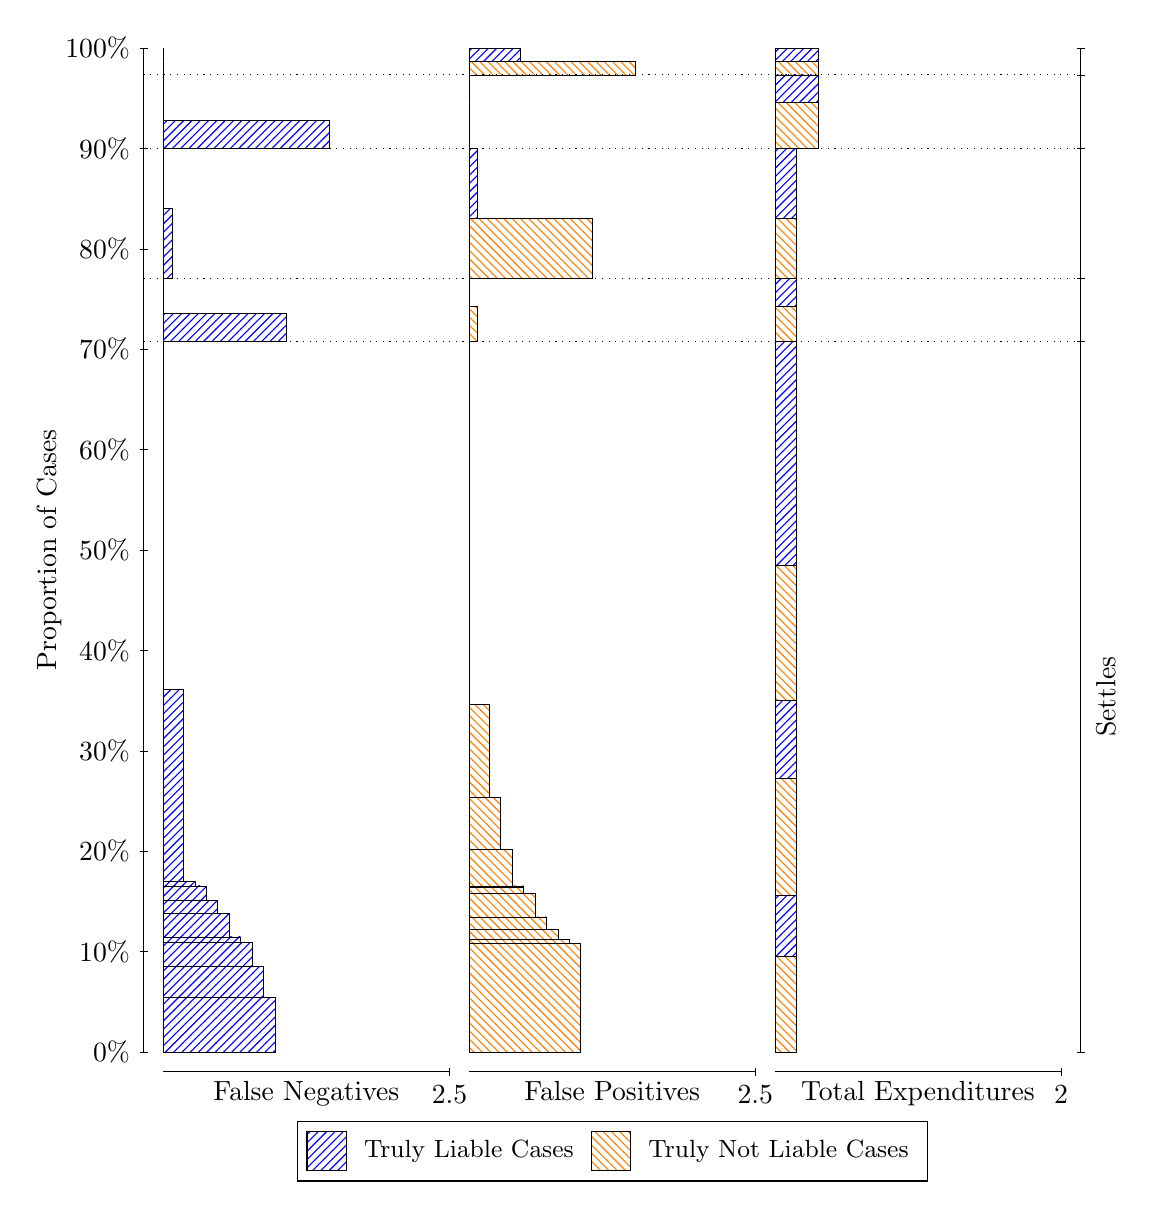
\begin{tikzpicture}
\draw[black, very thin] (1.5,1.75) -- (1.5,14.5);
\node[rotate=90, text=black, anchor=center] at (0.3, 8.125) {Proportion of Cases};
\draw[black, very thin] (1.45,1.75) -- (1.55,1.75);
\node[text=black, anchor=east] at (1.45, 1.75) {0\%};
\draw[black, very thin] (1.45,3.025) -- (1.55,3.025);
\node[text=black, anchor=east] at (1.45, 3.025) {10\%};
\draw[black, very thin] (1.45,4.3) -- (1.55,4.3);
\node[text=black, anchor=east] at (1.45, 4.3) {20\%};
\draw[black, very thin] (1.45,5.575) -- (1.55,5.575);
\node[text=black, anchor=east] at (1.45, 5.575) {30\%};
\draw[black, very thin] (1.45,6.85) -- (1.55,6.85);
\node[text=black, anchor=east] at (1.45, 6.85) {40\%};
\draw[black, very thin] (1.45,8.125) -- (1.55,8.125);
\node[text=black, anchor=east] at (1.45, 8.125) {50\%};
\draw[black, very thin] (1.45,9.4) -- (1.55,9.4);
\node[text=black, anchor=east] at (1.45, 9.4) {60\%};
\draw[black, very thin] (1.45,10.675) -- (1.55,10.675);
\node[text=black, anchor=east] at (1.45, 10.675) {70\%};
\draw[black, very thin] (1.45,11.95) -- (1.55,11.95);
\node[text=black, anchor=east] at (1.45, 11.95) {80\%};
\draw[black, very thin] (1.45,13.225) -- (1.55,13.225);
\node[text=black, anchor=east] at (1.45, 13.225) {90\%};
\draw[black, very thin] (1.45,14.5) -- (1.55,14.5);
\node[text=black, anchor=east] at (1.45, 14.5) {100\%};

\draw[black, very thin] (13.4,1.75) -- (13.4,14.5);
\draw[black, very thin] (13.35,1.75) -- (13.45,1.75);
\node[anchor=west] at (13.35, 1.75) {};
\draw[black, very thin] (13.35,10.773) -- (13.45,10.773);
\node[anchor=west] at (13.35, 10.773) {};
\draw[black, very thin] (13.35,11.57) -- (13.45,11.57);
\node[anchor=west] at (13.35, 11.57) {};
\draw[black, very thin] (13.35,13.225) -- (13.45,13.225);
\node[anchor=west] at (13.35, 13.225) {};
\draw[black, very thin] (13.35,14.159) -- (13.45,14.159);
\node[anchor=west] at (13.35, 14.159) {};
\draw[black, very thin] (13.35,14.5) -- (13.45,14.5);
\node[anchor=west] at (13.35, 14.5) {};

\draw[black, very thin, pattern color=blue, pattern=north east lines] (1.75,1.75) rectangle (3.167,2.4399);
\draw[black, very thin, pattern color=blue, pattern=north east lines] (1.75,2.4399) rectangle (3.0217,2.8372);
\draw[black, very thin, pattern color=blue, pattern=north east lines] (1.75,2.8372) rectangle (2.8763,3.1407);
\draw[black, very thin, pattern color=blue, pattern=north east lines] (1.75,3.1407) rectangle (2.731,3.2118);
\draw[black, very thin, pattern color=blue, pattern=north east lines] (1.75,3.2118) rectangle (2.5857,3.5075);
\draw[black, very thin, pattern color=blue, pattern=north east lines] (1.75,3.5075) rectangle (2.4403,3.6794);
\draw[black, very thin, pattern color=blue, pattern=north east lines] (1.75,3.6794) rectangle (2.295,3.8592);
\draw[black, very thin, pattern color=blue, pattern=north east lines] (1.75,3.8592) rectangle (2.1497,3.9183);
\draw[black, very thin, pattern color=blue, pattern=north east lines] (1.75,3.9183) rectangle (2.0043,6.3545);
\draw[black, very thin, pattern color=orange, pattern=north west lines] (1.75,6.3545) rectangle (1.75,10.773);
\draw[black, very thin, pattern color=blue, pattern=north east lines] (1.75,10.773) rectangle (3.3123,11.126);
\draw[black, very thin, pattern color=orange, pattern=north west lines] (1.75,11.126) rectangle (1.75,11.57);
\draw[black, very thin, pattern color=blue, pattern=north east lines] (1.75,11.57) rectangle (1.859,12.462);
\draw[black, very thin, pattern color=orange, pattern=north west lines] (1.75,12.462) rectangle (1.75,13.225);
\draw[black, very thin, pattern color=blue, pattern=north east lines] (1.75,13.225) rectangle (3.8573,13.578);
\draw[black, very thin, pattern color=orange, pattern=north west lines] (1.75,13.578) rectangle (1.75,14.159);
\draw[black, very thin, pattern color=orange, pattern=north west lines] (1.75,14.159) rectangle (1.75,14.327);
\draw[black, very thin, pattern color=blue, pattern=north east lines] (1.75,14.327) rectangle (1.75,14.5);
\draw[black, very thin, pattern color=orange, pattern=north west lines] (5.6333,1.75) rectangle (7.0503,3.1317);
\draw[black, very thin, pattern color=orange, pattern=north west lines] (5.6333,3.1317) rectangle (6.905,3.1755);
\draw[black, very thin, pattern color=orange, pattern=north west lines] (5.6333,3.1755) rectangle (6.7597,3.3095);
\draw[black, very thin, pattern color=orange, pattern=north west lines] (5.6333,3.3095) rectangle (6.6143,3.4649);
\draw[black, very thin, pattern color=orange, pattern=north west lines] (5.6333,3.4649) rectangle (6.469,3.7617);
\draw[black, very thin, pattern color=orange, pattern=north west lines] (5.6333,3.7617) rectangle (6.3237,3.8356);
\draw[black, very thin, pattern color=orange, pattern=north west lines] (5.6333,3.8356) rectangle (6.3237,3.8591);
\draw[black, very thin, pattern color=orange, pattern=north west lines] (5.6333,3.8591) rectangle (6.1783,4.3191);
\draw[black, very thin, pattern color=orange, pattern=north west lines] (5.6333,4.3191) rectangle (6.033,4.9792);
\draw[black, very thin, pattern color=orange, pattern=north west lines] (5.6333,4.9792) rectangle (5.8877,6.1686);
\draw[black, very thin, pattern color=blue, pattern=north east lines] (5.6333,6.1686) rectangle (5.6333,10.773);
\draw[black, very thin, pattern color=orange, pattern=north west lines] (5.6333,10.773) rectangle (5.7423,11.217);
\draw[black, very thin, pattern color=blue, pattern=north east lines] (5.6333,11.217) rectangle (5.6333,11.57);
\draw[black, very thin, pattern color=orange, pattern=north west lines] (5.6333,11.57) rectangle (7.1957,12.334);
\draw[black, very thin, pattern color=blue, pattern=north east lines] (5.6333,12.334) rectangle (5.7423,13.225);
\draw[black, very thin, pattern color=orange, pattern=north west lines] (5.6333,13.225) rectangle (5.6333,13.806);
\draw[black, very thin, pattern color=blue, pattern=north east lines] (5.6333,13.806) rectangle (5.6333,14.159);
\draw[black, very thin, pattern color=orange, pattern=north west lines] (5.6333,14.159) rectangle (7.7407,14.327);
\draw[black, very thin, pattern color=blue, pattern=north east lines] (5.6333,14.327) rectangle (6.2873,14.5);
\draw[black, very thin, pattern color=orange, pattern=north west lines] (9.5167,1.75) rectangle (9.7892,2.9675);
\draw[black, very thin, pattern color=blue, pattern=north east lines] (9.5167,2.9675) rectangle (9.7892,3.7394);
\draw[black, very thin, pattern color=orange, pattern=north west lines] (9.5167,3.7394) rectangle (9.7892,5.2256);
\draw[black, very thin, pattern color=blue, pattern=north east lines] (9.5167,5.2256) rectangle (9.7892,6.2113);
\draw[black, very thin, pattern color=orange, pattern=north west lines] (9.5167,6.2113) rectangle (9.7892,7.9261);
\draw[black, very thin, pattern color=blue, pattern=north east lines] (9.5167,7.9261) rectangle (9.7892,10.773);
\draw[black, very thin, pattern color=orange, pattern=north west lines] (9.5167,10.773) rectangle (9.7892,11.217);
\draw[black, very thin, pattern color=blue, pattern=north east lines] (9.5167,11.217) rectangle (9.7892,11.57);
\draw[black, very thin, pattern color=orange, pattern=north west lines] (9.5167,11.57) rectangle (9.7892,12.334);
\draw[black, very thin, pattern color=blue, pattern=north east lines] (9.5167,12.334) rectangle (9.7892,13.225);
\draw[black, very thin, pattern color=orange, pattern=north west lines] (9.5167,13.225) rectangle (10.062,13.806);
\draw[black, very thin, pattern color=blue, pattern=north east lines] (9.5167,13.806) rectangle (10.062,14.159);
\draw[black, very thin, pattern color=orange, pattern=north west lines] (9.5167,14.159) rectangle (10.062,14.327);
\draw[black, very thin, pattern color=blue, pattern=north east lines] (9.5167,14.327) rectangle (10.062,14.5);
\draw[black, dotted] (1.5,10.773) -- (13.4,10.773);
\draw[black, dotted] (1.5,11.57) -- (13.4,11.57);
\draw[black, dotted] (1.5,13.225) -- (13.4,13.225);
\draw[black, dotted] (1.5,14.159) -- (13.4,14.159);
\draw[black, very thin] (1.75,1.5) -- (5.3833,1.5);
\node[text=black, anchor=north] at (3.5667, 1.5) {False Negatives};
\draw[black, very thin] (5.3833,1.45) -- (5.3833,1.55);
\node[text=black, anchor=north] at (5.3833, 1.45) {2.5};

\draw[black, very thin] (5.6333,1.5) -- (9.2667,1.5);
\node[text=black, anchor=north] at (7.45, 1.5) {False Positives};
\draw[black, very thin] (9.2667,1.45) -- (9.2667,1.55);
\node[text=black, anchor=north] at (9.2667, 1.45) {2.5};

\draw[black, very thin] (9.5167,1.5) -- (13.15,1.5);
\node[text=black, anchor=north] at (11.333, 1.5) {Total Expenditures};
\draw[black, very thin] (13.15,1.45) -- (13.15,1.55);
\node[text=black, anchor=north] at (13.15, 1.45) {2};

\node[text=black, centered, rotate=90] at (13.72, 6.2615) {Settles};





\draw (7.449999999999999,1.5) node[draw=none] (baseCoordinate) {};
\begin{scope}[align=center]
        \matrix[scale=0.5, draw=black, below=0.5cm of baseCoordinate, nodes={draw}, column sep=0.1cm]{
            \node[rectangle, draw, minimum width=0.5cm, minimum height=0.5cm, pattern color=blue, pattern=north east lines] {}; &
            \node[draw=none, font=\small, text=black] (B) {Truly Liable Cases}; &
            \node[rectangle, draw, minimum width=0.5cm, minimum height=0.5cm, pattern color=orange, pattern=north west lines] {}; &
            \node[draw=none, font=\small, text=black] (B) {Truly Not Liable Cases}; \\
            };
\end{scope}

\end{tikzpicture}
\end{document}